                                                               %
\documentclass[pdflatex,sn-mathphys-num]{sn-jnl}

\usepackage{graphicx}%
\usepackage{multirow}%
\usepackage{amsmath,amssymb,amsfonts}%
\usepackage{amsthm}%
\usepackage{mathrsfs}%
\usepackage[title]{appendix}%
\usepackage{xcolor}%
\usepackage{textcomp}%
\usepackage{manyfoot}%
\usepackage{booktabs}%
\usepackage{algorithm}%
\usepackage{algorithmicx}%
\usepackage{algpseudocode}%
\usepackage{listings}%
\usepackage{bbm}%
\usepackage{subcaption}  % in preamble
\usepackage[section]{placeins}
%%%%

%%%%%=============================================================================%%%%
%%%%  Remarks: This template is provided to aid authors with the preparation
%%%%  of original research articles intended for submission to journals published 
%%%%  by Springer Nature. The guidance has been prepared in partnership with 
%%%%  production teams to conform to Springer Nature technical requirements. 
%%%%  Editorial and presentation requirements differ among journal portfolios and 
%%%%  research disciplines. You may find sections in this template are irrelevant 
%%%%  to your work and are empowered to omit any such section if allowed by the 
%%%%  journal you intend to submit to. The submission guidelines and policies 
%%%%  of the journal take precedence. A detailed User Manual is available in the 
%%%%  template package for technical guidance.
%%%%%=============================================================================%%%%

%% as per the requirement new theorem styles can be included as shown below
\theoremstyle{thmstyleone}%
\newtheorem{theorem}{Theorem}%  meant for continuous numbers
%%\newtheorem{theorem}{Theorem}[section]% meant for sectionwise numbers
%% optional argument [theorem] produces theorem numbering sequence instead of independent numbers for Proposition
\newtheorem{proposition}[theorem]{Proposition}% 
%%\newtheorem{proposition}{Proposition}% to get separate numbers for theorem and proposition etc.

\theoremstyle{thmstyletwo}%
\newtheorem{example}{Example}%
\newtheorem{remark}{Remark}%

\theoremstyle{thmstylethree}%
\newtheorem{definition}{Definition}%

\raggedbottom
%%\unnumbered% uncomment this for unnumbered level heads

\begin{document}

\title[Article Title]{Adaptive Bandit Algorithms for Drifting Users in Recommender Systems: A Comparative Study}

%%=============================================================%%
%% GivenName	-> \fnm{Joergen W.}
%% Particle	-> \spfx{van der} -> surname prefix
%% FamilyName	-> \sur{Ploeg}
%% Suffix	-> \sfx{IV}
%% \author*[1,2]{\fnm{Joergen W.} \spfx{van der} \sur{Ploeg} 
%%  \sfx{IV}}\email{iauthor@gmail.com}
%%=============================================================%%

\author*[1,2]{\fnm{Hema Chandra} \sur{Puchakayala}}\email{puchakayalahema@gmail.com}

\author[2,3]{\fnm{Second} \sur{Author}}\email{iiauthor@gmail.com}
\equalcont{These authors contributed equally to this work.}

\author[1,2]{\fnm{Third} \sur{Author}}\email{iiiauthor@gmail.com}
\equalcont{These authors contributed equally to this work.}

\affil*[1]{\orgdiv{Department}, \orgname{Organization}, \orgaddress{\street{Street}, \city{City}, \postcode{100190}, \state{State}, \country{Country}}}

\affil[2]{\orgdiv{Department}, \orgname{Organization}, \orgaddress{\street{Street}, \city{City}, \postcode{10587}, \state{State}, \country{Country}}}

\affil[3]{\orgdiv{Department}, \orgname{Organization}, \orgaddress{\street{Street}, \city{City}, \postcode{610101}, \state{State}, \country{Country}}}

%%==================================%%
%% Sample for unstructured abstract %%
%%==================================%%

\abstract{Recommender systems deployed in dynamic environments must adapt to users whose preferences drift over time, yet many bandit algorithms still assume stationary reward distributions. This work presents a reproducible simulation framework that models user drift as a latent preference vector over content categories evolving in a non-stationary multi-armed bandit setting. Within this framework we implement four adaptive algorithms—Non-Stationary $\varepsilon$-Greedy, Sliding-Window UCB, CUSUM-UCB, and EXP3.S—and evaluate them on synthetically generated drifting-user data using average and cumulative reward with confidence intervals over 50 runs. The results show that Sliding-Window UCB consistently achieves the highest long-run reward, followed by CUSUM-UCB and Non-Stationary $\varepsilon$-Greedy, while the adversarially robust EXP3.S underperforms in this stochastic drift regime. These findings suggest that methods which explicitly discount or reset outdated observations are well suited to gradual user drift, and that adversarial bandit algorithms can be overly conservative when non-stationarity arises from user behavior rather than malicious manipulation.}


\keywords{Non-stationary multi-armed bandits, User preference drift, Recommender systems, Sliding-Window UCB, CUSUM-UCB, Non-stationary epsilon-greedy, EXP3.S adversarial bandit, Exploration–exploitation trade-off}

%%\pacs[JEL Classification]{D8, H51}

%%\pacs[MSC Classification]{35A01, 65L10, 65L12, 65L20, 65L70}

\maketitle

\section{Introduction}\label{sec1}

Modern recommender systems must adapt to users whose preferences change over time, a phenomenon commonly referred to as user drift.
% Traditional reinforcement learning models such as Q-learning rely on the assumption that actions taken by the agent influence the state of the environment. Many recommendation scenarios do not satisfy this assumption because 
User preferences change independently of the system’s actions. When the environment evolves on its own rather than through action-induced state transitions, the problem aligns more closely with a non-stationary multi-armed bandit setting rather than a multi-state Markov decision process.

To investigate this class of problems in a controlled and reproducible manner, this research constructs synthetic user environments in which each user is represented by a latent preference vector over a set of content categories or arms. In the initial timestep, users begin without inherent bias between arms, matching the initialization used in the drift environment defined in env.py. These latent vectors determine the initial affinities of each user and serve as the basis for reward generation.

User drift is simulated by updating each user’s latent affinity vector at every timestep. The vector is normalized to preserve a valid normal probability distribution. This process captures gradual or abrupt changes in user interest that occur naturally in real-world applications due to evolving tastes, external trends, or shifting contexts. Importantly, this drift occurs independently of the agent’s actions, which reinforces the interpretation of the recommendation task as a single-state non-stationary bandit problem.

Because user preferences evolve over time, algorithms must adapt quickly to changes in reward distributions. This study evaluates four adaptive bandit algorithms: Non-Stationary Epsilon-Greedy, Sliding Window UCB (SW-UCB), CUSUM-UCB, and EXP3.S. Each algorithm processes the same synthetically generated datasets that include drift in user preferences. This controlled setup ensures reproducibility and creates a fair basis for performance comparison. The objective is to examine how effectively each algorithm can detect and track the shifting reward landscape and to determine which methods are most suitable for recommendation tasks in dynamic environments.


\section{Literature Review}\label{sec2}

% ALL PREVIOUS MODELS HERE (bullet point with short description)
A wide range of strategies has been developed to address non-stationarity in
multi-armed bandit problems, particularly in settings where the reward distribution
drifts or changes abruptly over time. Classical bandit algorithms such as UCB and
$\varepsilon$-greedy assume stationary reward distributions and therefore struggle when
user preferences evolve, as their estimates place equal weight on outdated and recent
observations. To mitigate this limitation, several adaptive variants have been proposed
in the literature, each incorporating mechanisms to discount stale information, detect
distributional shifts, or explicitly reset statistics after suspected changes.

This section reviews four representative approaches that form the basis of our
comparative study: Sliding-Window UCB (SW-UCB), Non-Stationary
$\varepsilon$-Greedy, EXP3.S, and CUSUM-UCB. These methods span both stochastic
and adversarial formulations of non-stationary bandits and provide a spectrum of
adaptation mechanisms, including sliding-window averaging, exponential
recency-weighted updates, weight-sharing regularization, and online change detection.
By examining these algorithms, we establish a comprehensive foundation for evaluating 
how different adaptation strategies respond to user drift in recommendation-style 
environments.

\begin{itemize}

    % \item \textbf{LinUCB}\cite{linucb}:  
    % LinUCB is a contextual bandit algorithm that assumes a linear relationship between context features and expected rewards.  
    % For each arm $a$, LinUCB maintains an estimate of a parameter vector $\theta_a$ such that  
    % \[
    %     \mathbb{E}[r_t(a)] = x_t^\top \theta_a.
    % \]  
    % The action-selection rule uses an upper-confidence bound:  
    % \[
    %     a_t = \arg\max_a \; x_t^\top \hat{\theta}_a + \alpha \sqrt{x_t^\top A_a^{-1} x_t},
    % \]
    % where $A_a = D_a^\top D_a + I$ is the covariance matrix and $b_a = \sum r_i x_i$. The parameter estimate is  
    % \[
    %     \hat{\theta}_a = A_a^{-1} b_a. 
    % \]  
    % After observing reward $r_t$, updates are  
    % \[
    %     A_a \leftarrow A_a + x_t x_t^\top, \qquad b_a \leftarrow b_a + r_t x_t.
    % \]

    \item \textbf{Sliding-Window UCB (SW-UCB)}\cite{swucb}:  
    SW-UCB is a variant of UCB designed for non-stationary environments with abrupt changes.  
    Instead of using all past observations, it computes estimates using only the most recent $\tau$ rounds, 
    allowing rapid adaptation to changing reward distributions.  

    The sliding-window empirical mean for arm $i$ at time $t$ is  
    \[
        \bar{X}_t(\tau, i)
        = \frac{1}{N_t(\tau, i)}
        \sum_{s = t-\tau+1}^{t} X_s(i)\,\mathbbm{1}_{\{I_s = i\}},
    \]
    where  
    \[
    N_t(\gamma,i) \;=\; \sum_{s=1}^{t} \gamma^{\,t-s}\,\mathbbm{1}_{\{I_s = i\}},
    \]
 The is the number of times the arm $i$ was selected in the last $\tau$ rounds, $\gamma \in (0,1)$ is the discount factor controlling how quickly past observations are forgotten and $\xi$ is a some appropriate constant.

    SW-UCB constructs an upper-confidence bound using:  
    \[
        c_t(\tau, i)
        = B \sqrt{\frac{\xi \log (t \wedge \tau)}{N_t(\tau, i)}},
    \]
    where $B$ is the upper-bound on the rewards, $t \wedge \tau$ denotes the minimum of t and $\tau$ and $\xi > 1/2$ controls exploration.

    \textbf{Action selection is performed by}\\
\quad for $t = 1$ to $K$, play arm $I_t = t$;\\
\quad for $t = K+1$ to $T$, play arm
\[
    I_t
    = \arg\max_{1 \le i \le K}
    \left(
        \bar{X}_t(\tau,i) + c_t(\tau,i)
    \right).
\]

    After receiving the reward $X_t(a_t)$, the sliding-window statistics are updated by discarding observations older than $\tau$ rounds and inserting the new one:
    \[
        N_{t+1}(\gamma, i)
        = \sum_{s = t-\tau+2}^{t+1} \gamma^{\,t+1-s}\, \mathbbm{1}_{\{I_s = i\}},
    \]
    \[
        \bar{X}_{t+1}(\tau, a)
        = \frac{1}{N_{t+1}(\tau, a)}
          \sum_{s = t-\tau+2}^{t+1} X_s(i)\,\mathbbm{1}_{\{I_s = i\}},
    \]
    \[
        c_{t+1}(\tau, i)
        = B \sqrt{\frac{\xi \log((t+1) \wedge \tau)}{N_{t+1}(\tau, i)}}.
    \]

    \item \textbf{Non-Stationary Epsilon-Greedy}\cite{epsilon_greedy_ns}: 
    This is an adaptation of the classical $\varepsilon$-greedy method for
    environments in which the reward distributions drift over time.  
    Instead of sample averages, the action-value estimates use a
    \emph{constant step-size} update, which implements an
    exponential recency-weighted average that discounts older rewards.

    The estimate of the value of arm $i$ at time $t$ is updated according to
    the incremental constant–step-size rule  
    \[
        Q_{t+1}(i)
        \;=\;
        Q_t(i)
        \;+\;
        \alpha\Big(R_t - Q_t(i)\Big)\,\mathbbm{1}_{\{I_t = i\}},
    \]
    where $\alpha \in (0,1]$ is the constant step-size parameter.  
    Unrolling this recursion gives the exponential recency-weighted form
    \[
        Q_{t+1}(i)
        \;=\;
        (1-\alpha)^{t} Q_1(i)
        \;+\;
        \sum_{s=1}^{t}
        \alpha(1-\alpha)^{t-s}\,R_s\,\mathbbm{1}_{\{I_s=i\}},
    \]
    showing that recent rewards receive more weight than older ones, with
    decay factor $(1-\alpha)$.

    \textbf{Action selection is performed using} the $\varepsilon$-greedy policy:\\
\quad for $t = 1$ to $K$, play arm $I_t = t$;\\
\quad for $t = K+1$ to $T$, select arm
    \[
        I_t
        =
        \begin{cases}
            \text{a random arm in }\{1,\dots,K\}, & \text{with probability }\varepsilon, \\[6pt]
            \displaystyle \arg\max_{1\le i\le K} Q_t(i),     & \text{with probability }1-\varepsilon.
        \end{cases}
    \]

    After observing reward $R_t$, the value estimates are updated using the
    constant step-size rule:
    \[
        Q_{t+1}(I_t)
        =
        Q_t(I_t)
        +
        \alpha\,\big(R_t - Q_t(I_t)\big).
    \]

    Because the estimate $Q_t(i)$ places exponentially decaying weight on past
    rewards with weights proportional to $(1-\alpha)^k$ for $k$-step-old
    observations method adapts effectively to non-stationary reward
    distributions. Larger values of $\alpha$ allow faster adaptation, while
    smaller values provide greater stability.

    \item \textbf{EXP3.S}\cite{exp3s}:  
EXP3.S is a variant of the EXP3 algorithm proposed in Auer et al. (1995) \cite{exp3} designed to control regret against \emph{arbitrary} (possibly switching) action sequences.
Rather than competing only with the best single arm, EXP3.S adapts to
piecewise-stationary environments by incorporating an additional
stabilization term in the weight update that helps the algorithm track
changing optimal arms.

Like EXP3, it maintains exponential weights over the $K$ arms and mixes
between exploitation and uniform exploration.  
However, EXP3.S adds a regularization term proportional to 
$\alpha$ that penalizes rapid fluctuations and allows regret bounds
scaling with the \emph{hardness} of the comparator sequence (i.e., the number of switches throughout the sequence).

\vspace{4pt}
\textbf{Action selection:}\\
\quad At each round $t$, compute the probability distribution
\[
    p_i(t)
    \;=\;
    (1-\gamma)\,
    \frac{w_i(t)}{\sum_{j=1}^K w_j(t)}
    \;+\;
    \frac{\gamma}{K},
    \qquad i=1,\dots,K.
\]
\quad Then draw action $I_t$ according to the distribution $p(t)$.

\vspace{4pt}
\textbf{Reward estimation:}\\
After receiving reward $x_{I_t}(t) \in [0,1]$, define the unbiased
importance-weighted estimator
\[
    \widehat{x}_j(t)
    \;=\;
    \begin{cases}
        \displaystyle \frac{x_j(t)}{p_j(t)}, & j = I_t,\\[6pt]
        0, & j \neq I_t .
    \end{cases}
\]

\vspace{4pt}
\textbf{Weight update:}\\
For each arm $j = 1,\dots,K$, update
\[
    w_j(t+1)
    \;=\;
    w_j(t)\,
    \exp\!\left(\frac{\gamma}{K}\,\widehat{x}_j(t)\right)
    \;+\;
    \frac{e{\alpha}}{K}
    \sum_{i=1}^K w_i(t).
\]

The additive term
\[
    \frac{e{\alpha}}{K}\sum_{i=1}^K w_i(t)
\]
helps the algorithm adapt to environments where the best arm switches,
enabling regret bounds that depend on the number of switches rather than on~$T$ alone.


\item \textbf{CUSUM-UCB}\cite{cusumucb}:
CUSUM-UCB is a change–detection based bandit algorithm designed for
piecewise-stationary environments. It augments the classical UCB index
with a two-sided online CUSUM detector that monitors each arm for
statistically significant shifts in its reward distribution. When a
change is detected on arm $i$, the algorithm \emph{restarts} that arm by
resetting its empirical mean, sample count, and the associated CUSUM
statistics. This prevents outdated pre-change rewards from contaminating
the UCB estimate and enables rapid recovery after abrupt changes.
For each arm, the first $M$ observations are used to estimate the
pre-change mean,
\[
\hat u_0 \;=\; \frac{1}{M}\sum_{k=1}^{M} y_k,
\]
and for each subsequent sample $y_k$, the CUSUM updates use the steps
\[
(s_k^+, s_k^-) \;=\; (y_k - \hat u_0 - \varepsilon,\;\; \hat u_0 - y_k - \varepsilon)\,\mathbbm{1}_{\{k > M\}},
\]
\[
g_k^+ = \max\{0,\; g_{k-1}^+ + s_k^+\}, \qquad 
g_k^- = \max\{0,\; g_{k-1}^- + s_k^-\}.
\]
A change is detected whenever either statistic crosses the threshold $h$,
i.e.,
\[
g_k^+ \ge h \quad \text{or} \quad g_k^- \ge h,
\]
upon which the corresponding arm is restarted:
its restart time $\tau_i$ is set to the current round, and the CUSUM
variables $(g_k^+, g_k^-)$ are reset to zero.

The UCB part of the algorithm uses only post-restart statistics.
Let $\tau_i$ denote the last restart time of arm $i$. Then its valid
sample count, empirical mean, and confidence padding at time $t$ are
\[
N_t(i) = \sum_{s=\tau_i}^{t} \mathbbm{1}_{\{I_s = i\}}, \qquad
\bar X_t(i) = \frac{1}{N_t(i)}\sum_{s=\tau_i}^{t} X_s(i)\,\mathbbm{1}_{\{I_s = i\}},
\]
\[
C_t(i) = \sqrt{\frac{\xi \log n_t}{N_t(i)}}, \qquad
n_t = \sum_{j=1}^{K} N_t(j),
\]
where $\xi > 0$ is the UCB exploration constant.

\textbf{Action selection} combines UCB exploitation with uniform
sampling at rate $\alpha$, as required to feed the CUSUM detectors:
\[
I_t = 
\begin{cases}
\displaystyle \arg\max_{1\le i\le K}\bigl(\bar X_t(i) + C_t(i)\bigr), & \text{with probability } 1 - \alpha,\\[8pt]
\text{a uniformly random arm in }\{1,\dots,K\}, & \text{with probability } \alpha/K.
\end{cases}
\]

\textbf{Update rule:}
After observing reward $X_t(I_t)$, the algorithm
\begin{enumerate}
\item updates the CUSUM statistics $g_k^+,g_k^-,s_k^+,s_k^-$ for the played arm;
\item if a CUSUM alarm is raised, resets $\tau_{I_t}=t+1$ and clears the CUSUM state;
\item otherwise, updates $(N_t(i),\bar X_t(i),C_t(i))$ for the played arm using the post-restart definitions above.
\end{enumerate}
Because all pre-change samples of an arm are discarded upon detection,
CUSUM-UCB avoids the slow recovery faced by classical UCB when reward
means abruptly decrease. 
\end{itemize}

   



% **Start here** just list previous work and BibTex 

% \quad LinUCB\cite{linucb} 

% ALL PREVIOUS MODELS HERE (bullet point with a short paragraph description of each model)

% \begin{itemize}
%     \item LinUCB\cite{linucb}: ADD DESCRIPTION HERE AND ACTION SELECTION FUNCTIONS AND UPDATE FUNCTIONS \\ 
%     \item EXP.S\cite{linucb}: ADD ....
% \end{itemize}

\section{Methodology}\label{sec3}

\subsection{Bandit Framework}\label{sec3-1}



All experiments are conducted in the \texttt{drifting} user environment generated
by the \texttt{create\_environment} function, where a single user’s preference
vector over \(K\) documents evolves over time through Gaussian perturbations and
renormalization. The number of arms is fixed to \(K = 2\), corresponding to two
competing documents, and each episode consists of \(T = 10{,}000\) interaction
steps. For every algorithm, performance is estimated over \(50\) independent
experiments, each initialized with a distinct random seed drawn from
\(\{0,\dots,99\}\).\cite{swucb,epsilon_greedy_ns,cusumucb,exp3s}

For each model and seed, the runner first samples a new drifting user trajectory,
then trains the selected bandit policy with its prescribed hyperparameters
(Non-Stationary \(\varepsilon\)-Greedy with \(\varepsilon = 0.05\) and
\(\alpha = 0.001\); SW-UCB with window size \(50\); CUSUM-UCB with
\(\varepsilon = 0.2\), \(h = 10\), \(\alpha = 0.2\); EXP3.S with
\(\gamma = 0.07\), \(\alpha = 0.1\)). At each round the environment emits a
reward vector, the agent selects one arm, and only the realized reward on that arm
is observed and logged together with a one-hot encoding of the chosen action.

After every run, three NumPy arrays are saved per model and seed: the underlying
reward data, the sequence of observed rewards, and a matrix of arm selections.
These tensors are later aggregated across all \(50\) trials to compute mean rolling
averages and cumulative rewards, as well as corresponding pointwise \(95\%\)
confidence intervals that are visualized in Figures~\ref{fig:bandit-avg-reward}
and~\ref{fig:bandit-cum-reward}


\begin{figure}[htbp]
    \centering
    % first plot: rolling average
    \begin{subfigure}[t]{0.95\linewidth}
        \centering
        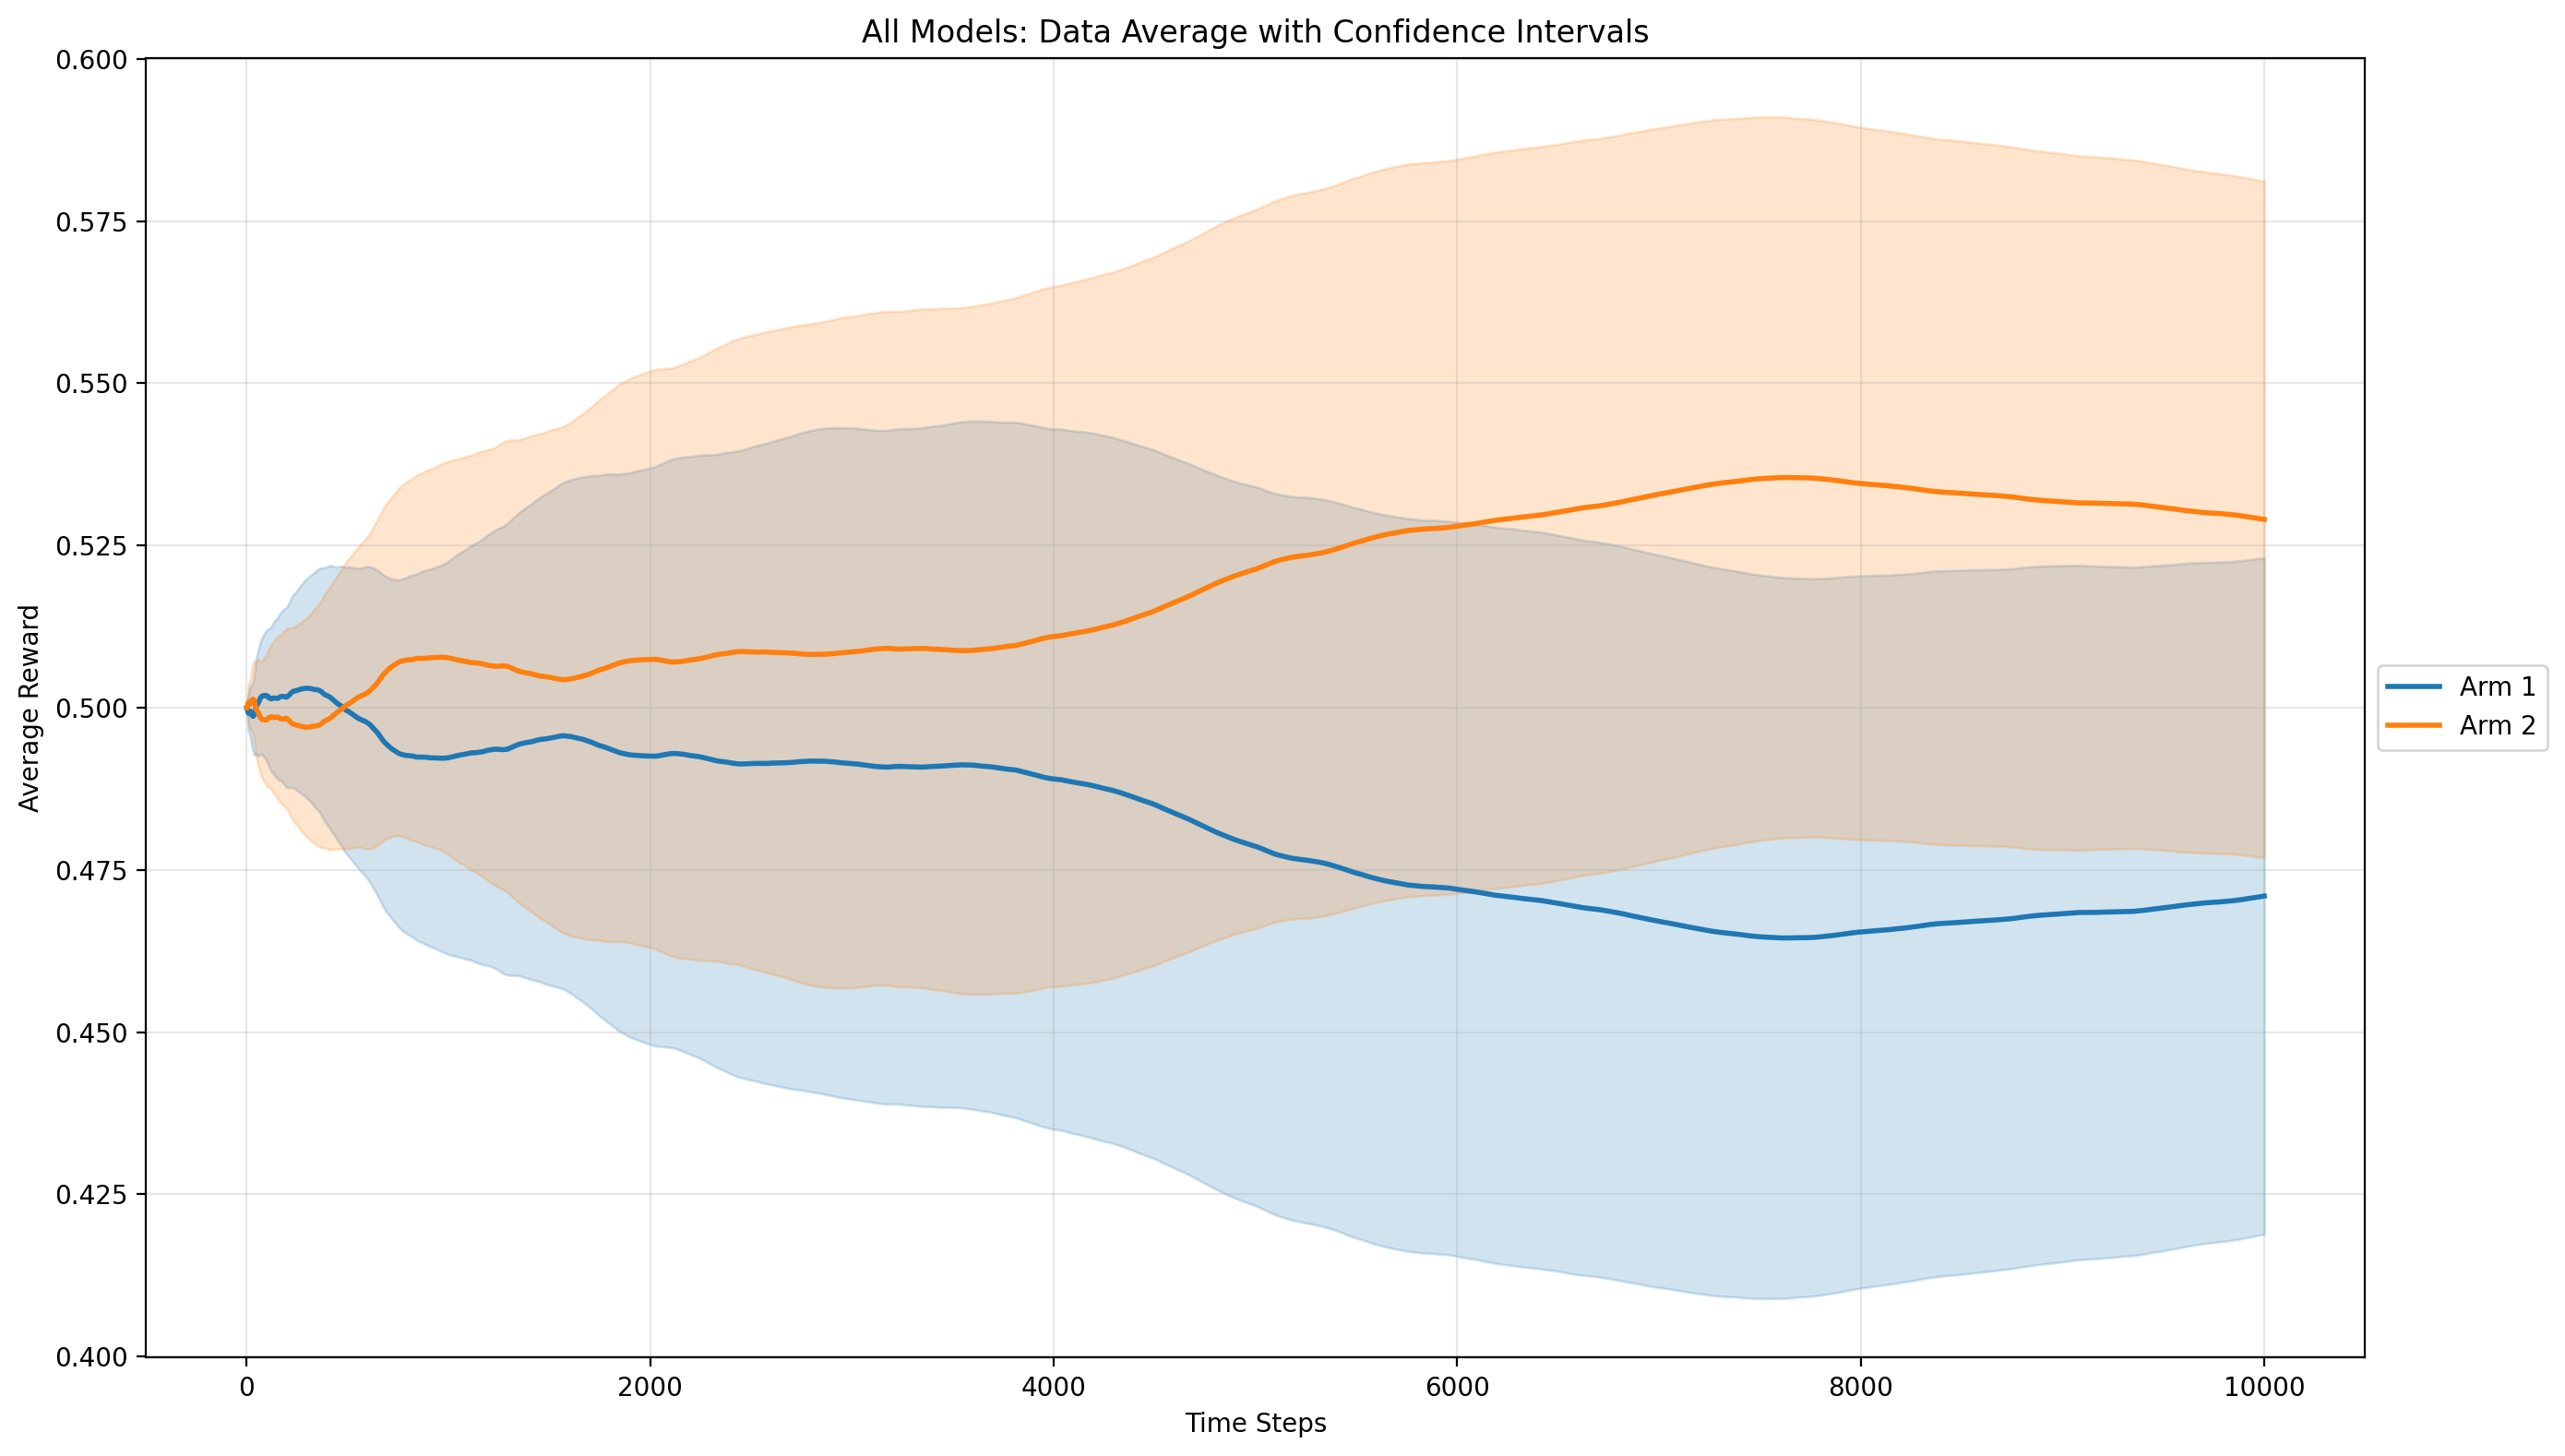
\includegraphics[width=\linewidth]{Fig/all_models_average_ci.png}
        \caption{Rolling average reward of each arm over $T=10{,}000$ rounds in the drifting user environment. The solid lines show the mean per–time‑step reward across $50$ runs, with shaded $95\%$ confidence intervals.}
        \label{fig:bandit-avg-reward}
    \end{subfigure}

    \vspace{0.5em}

    % second plot: cumulative reward
    \begin{subfigure}[t]{0.95\linewidth}
        \centering
        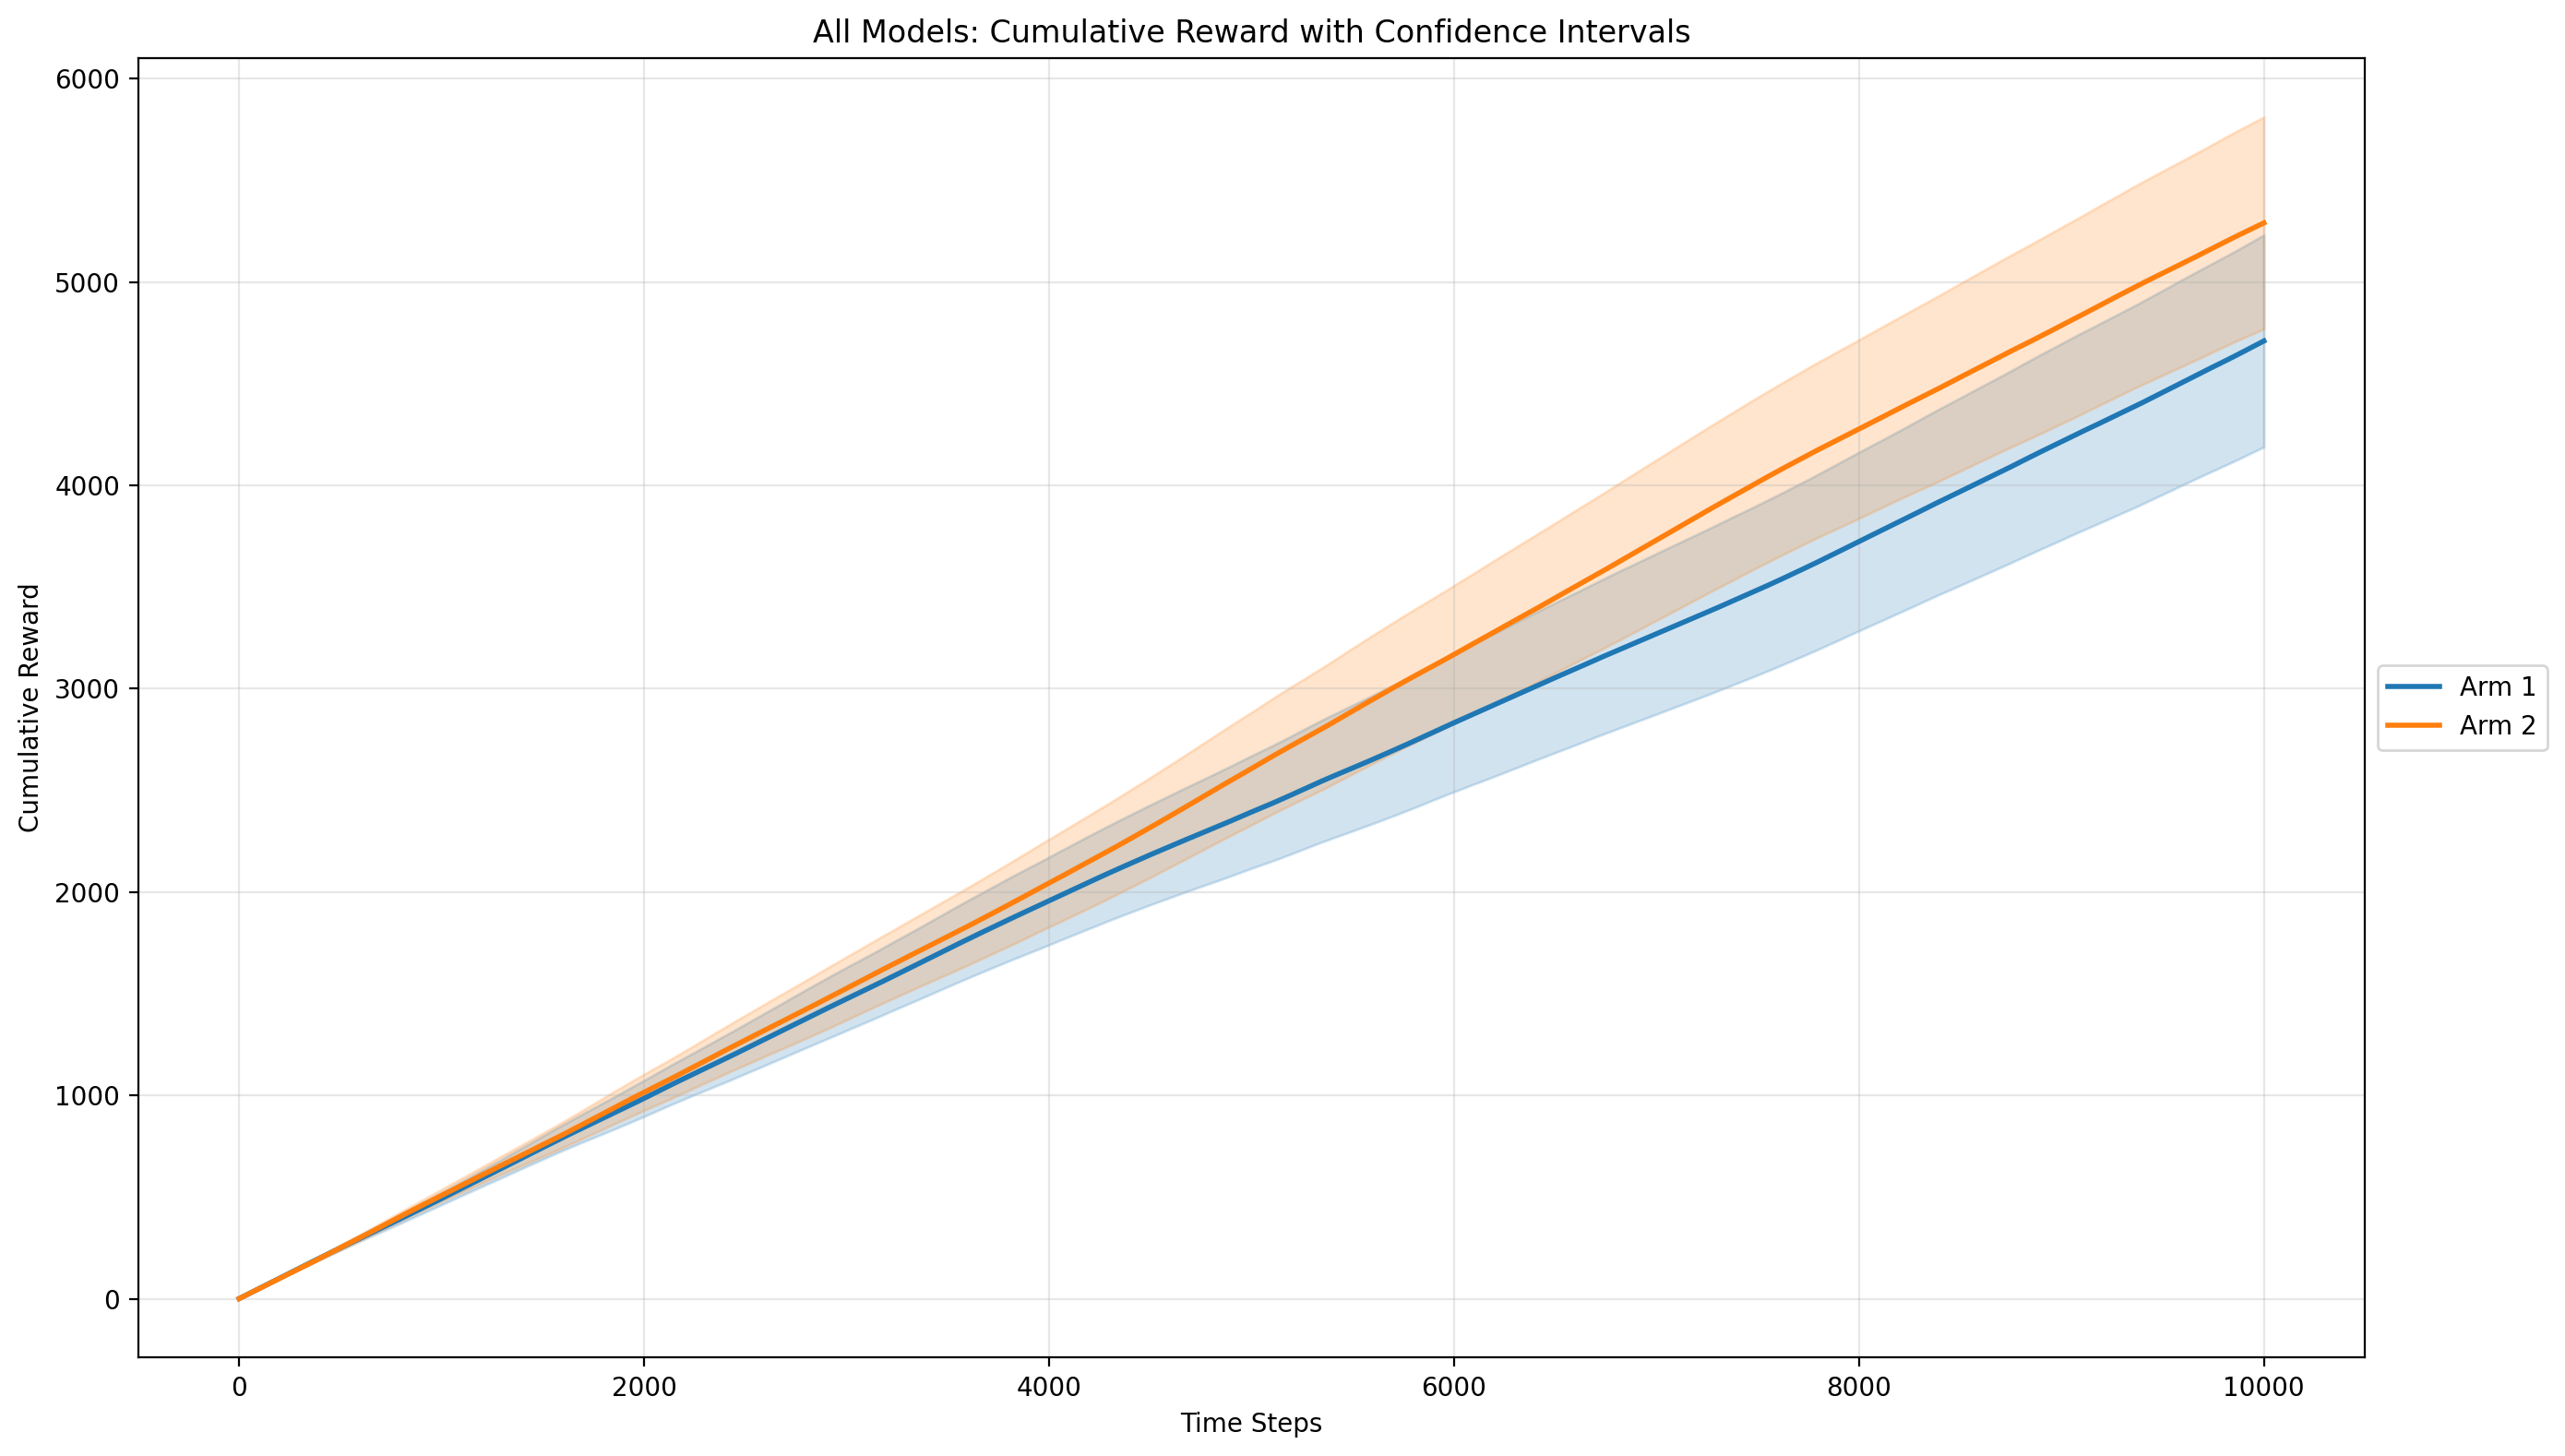
\includegraphics[width=\linewidth]{Fig/all_models_cumulative_ci.png}
        \caption{Cumulative reward of each arm over $T=10{,}000$ rounds. The mean cumulative reward across $50$ runs is shown with shaded $95\%$ confidence intervals, highlighting that Arm~2 becomes dominant as preferences drift.}
        \label{fig:bandit-cum-reward}
    \end{subfigure}

    \caption{Drifting user environment: average and cumulative rewards for both arms with confidence intervals.}
    \label{fig:bandit-environment}
\end{figure}

\FloatBarrier

\subsection{Metrics}\label{sec3-3}

The primary objective metric is \emph{cumulative reward}, defined for a policy
\(\pi\) over horizon \(T\) as
\[
R_{\text{cum}}^\pi(T)
=
\sum_{t=1}^{T} R_t,
\]
where \(R_t\) is the realized reward at round \(t\). This quantity captures the
total utility accrued by the algorithm and is the standard notion of
performance in bandit settings. For each model, we report the mean and
pointwise \(95\%\) confidence intervals of \(R_{\text{cum}}^\pi(T)\) across the
50 independent runs generated in our experimental setup.\cite{swucb,epsilon_greedy_ns,cusumucb,exp3s}

To analyze adaptation speed and stability, we also consider the \emph{rolling
average reward}
\[
\bar{R}^\pi(t)
=
\frac{1}{t}\sum_{s=1}^{t} R_s,
\qquad t = 1,\dots,T,
\]
which summarizes the per–time-step performance up to round \(t\). The rolling
average highlights transient behavior during regime changes, while the
cumulative curve emphasizes long-run efficiency. In both cases, we aggregate
results over random seeds and estimate confidence bands using the empirical
standard error, similar to visualization in Figures~\ref{fig:bandit-avg-reward}
and~\ref{fig:bandit-cum-reward}.


\section{Results}\label{sec4}

Figure~\ref{fig:bandit-environment}\,(a) shows that all stochastic bandit algorithms
quickly improve their average reward as they adapt to the drifting user
preferences, but they do so at different rates. SlidingWindowUCB exhibits the
fastest increase and ultimately attains the highest steady-state performance,
followed by CUSUM-UCB and the Non-Stationary \(\varepsilon\)-Greedy baseline.
EXP3.S, which is tailored to adversarial settings, improves more slowly and
stabilizes at a noticeably lower average reward.

The cumulative reward curves in Figure~\ref{fig:bandit-environment}\,(b) reflect
the same ordering. SlidingWindowUCB accumulates the largest total reward over
the \(10{,}000\) rounds, confirming its advantage in this smoothly drifting
environment, while CUSUM-UCB and Non-Stationary \(\varepsilon\)-Greedy achieve
similar but slightly smaller gains. EXP3.S lags behind throughout the horizon,
indicating that its robustness to adversarial sequences comes at the cost of
lower efficiency when the rewards are stochastic but non-stationary.


\begin{figure}[htbp]
    \centering
\centering
    % (a) Average reward
    \begin{subfigure}[t]{0.95\linewidth}
        \centering
        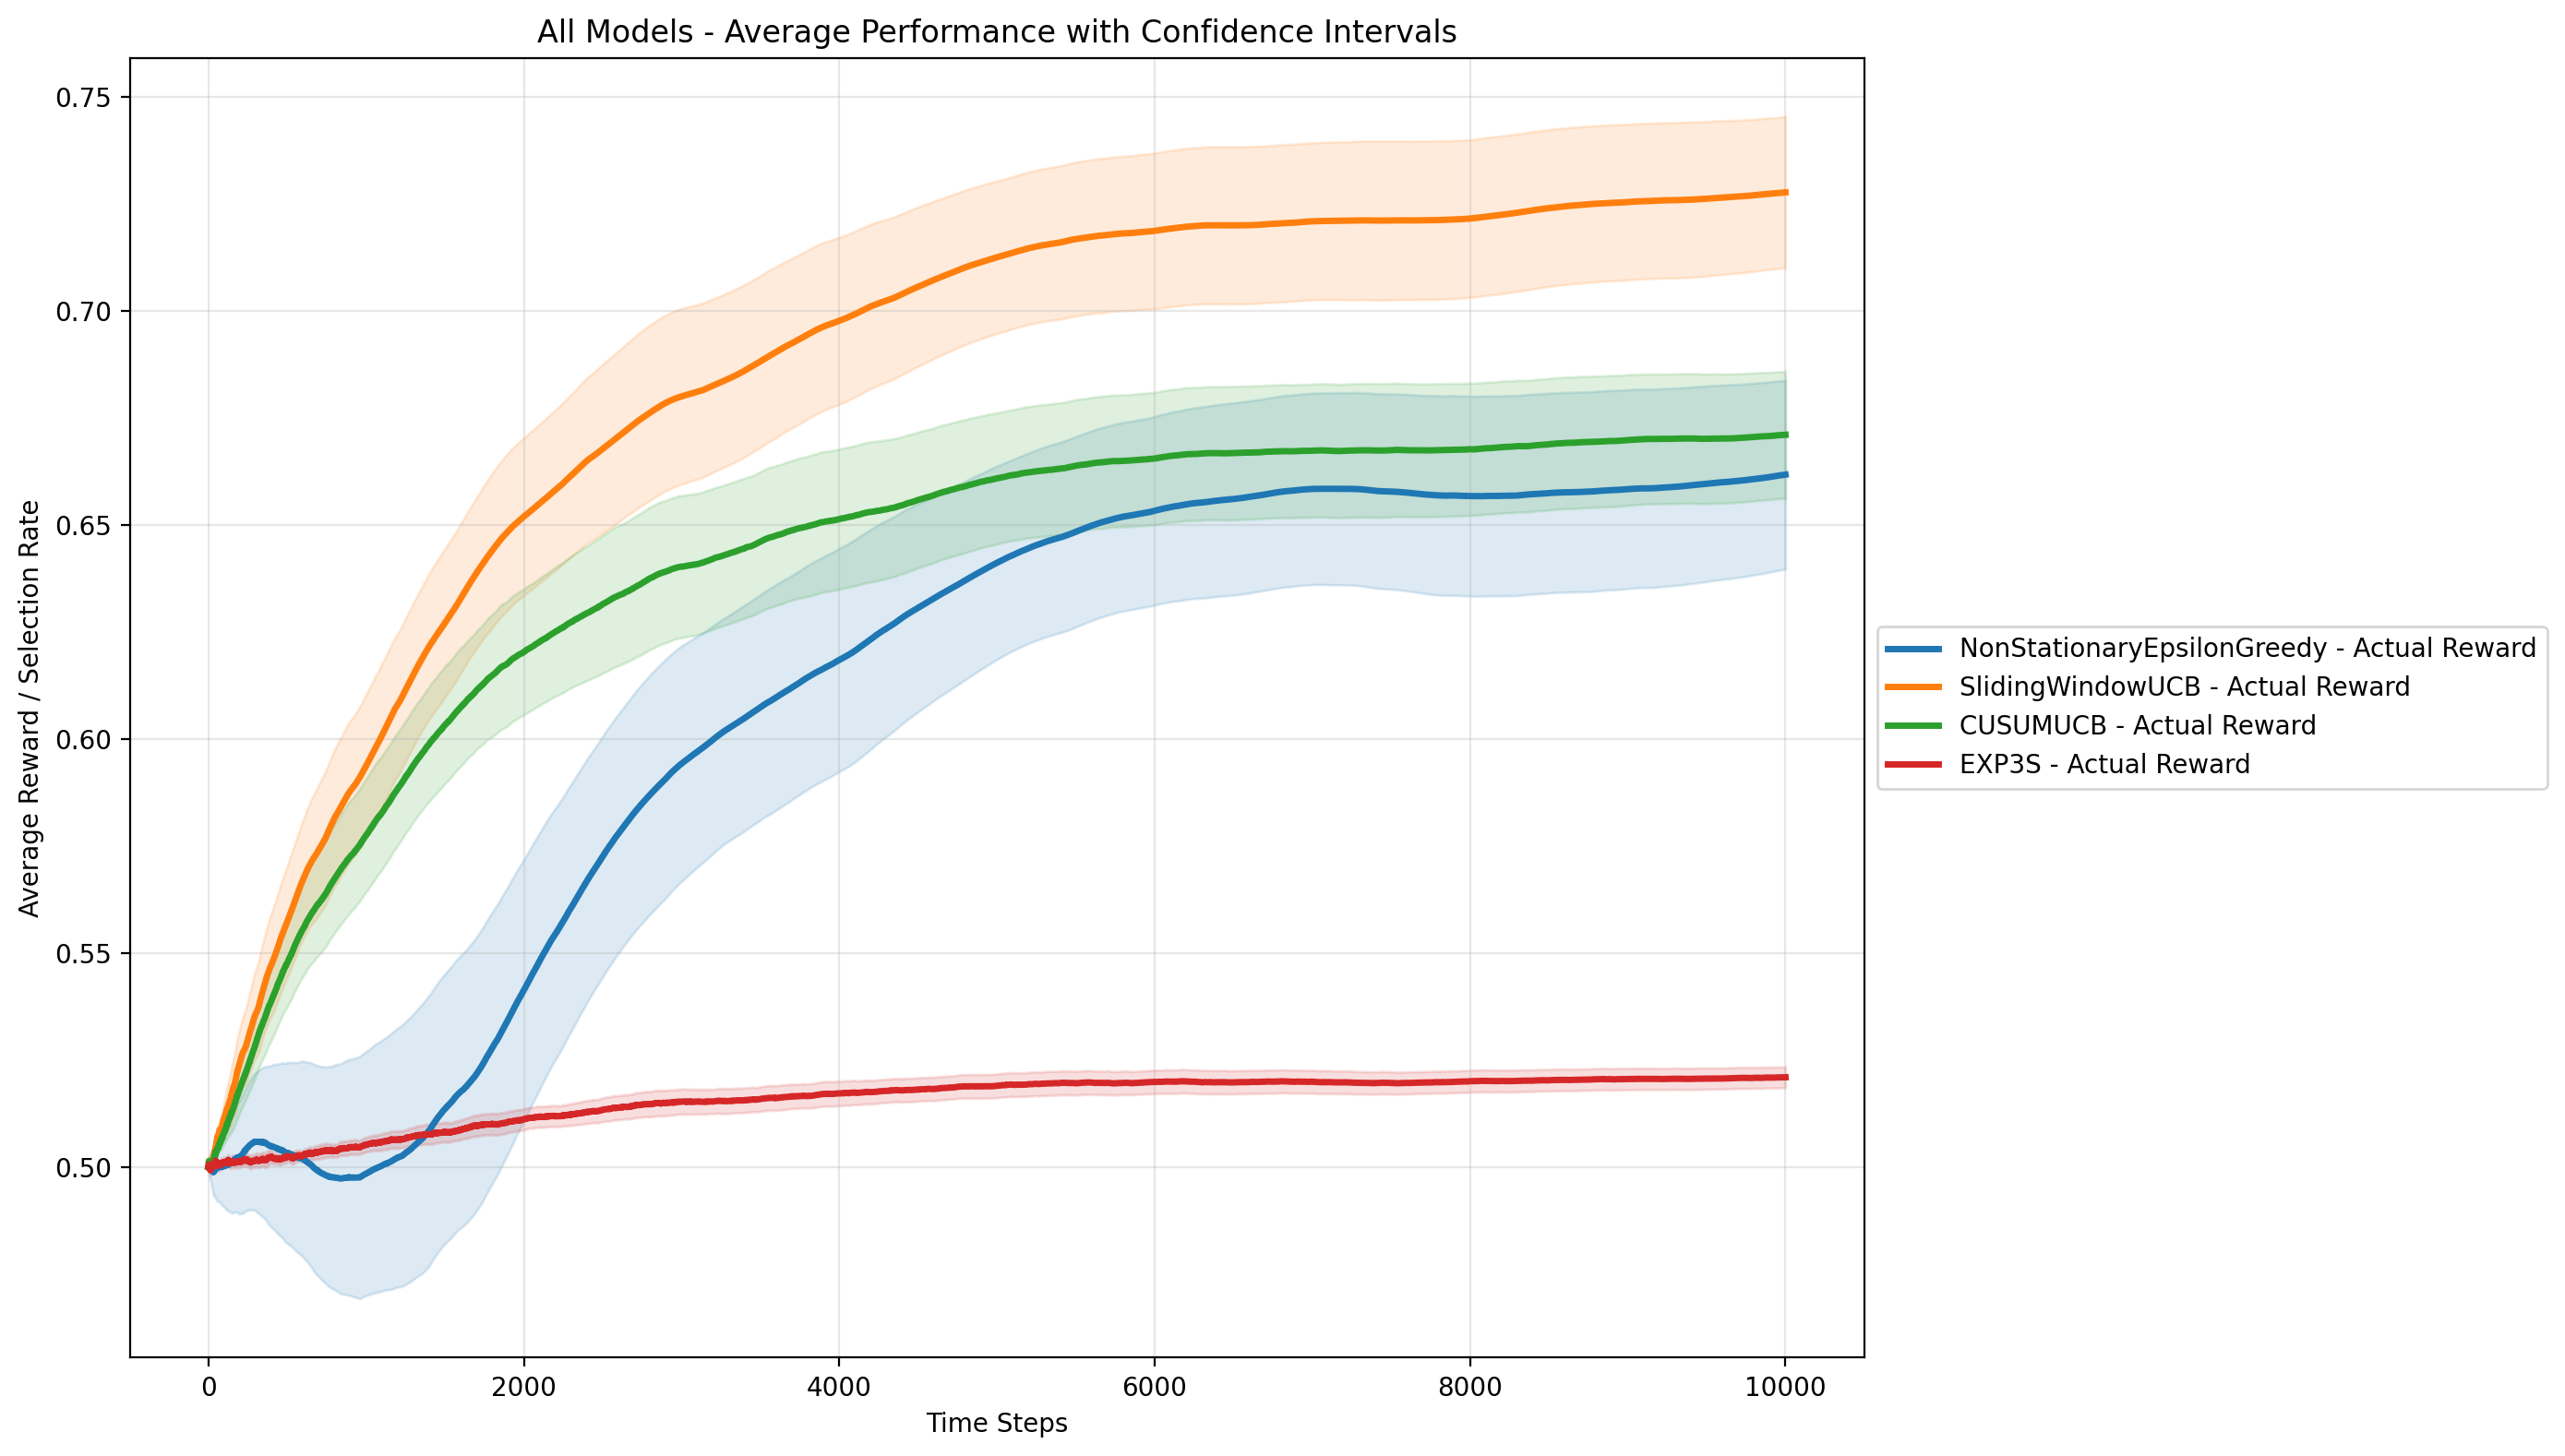
\includegraphics[width=\linewidth]{Fig/model_average_all_ci.png}
        \caption{Mean rolling average reward for all four algorithms over \(T = 10{,}000\) rounds, averaged across \(50\) runs with pointwise \(95\%\) confidence intervals.}
        \label{fig:models-avg-reward}
    \end{subfigure}

    \vspace{0.5em}

    % (b) Cumulative reward
    \begin{subfigure}[t]{0.95\linewidth}
        \centering
        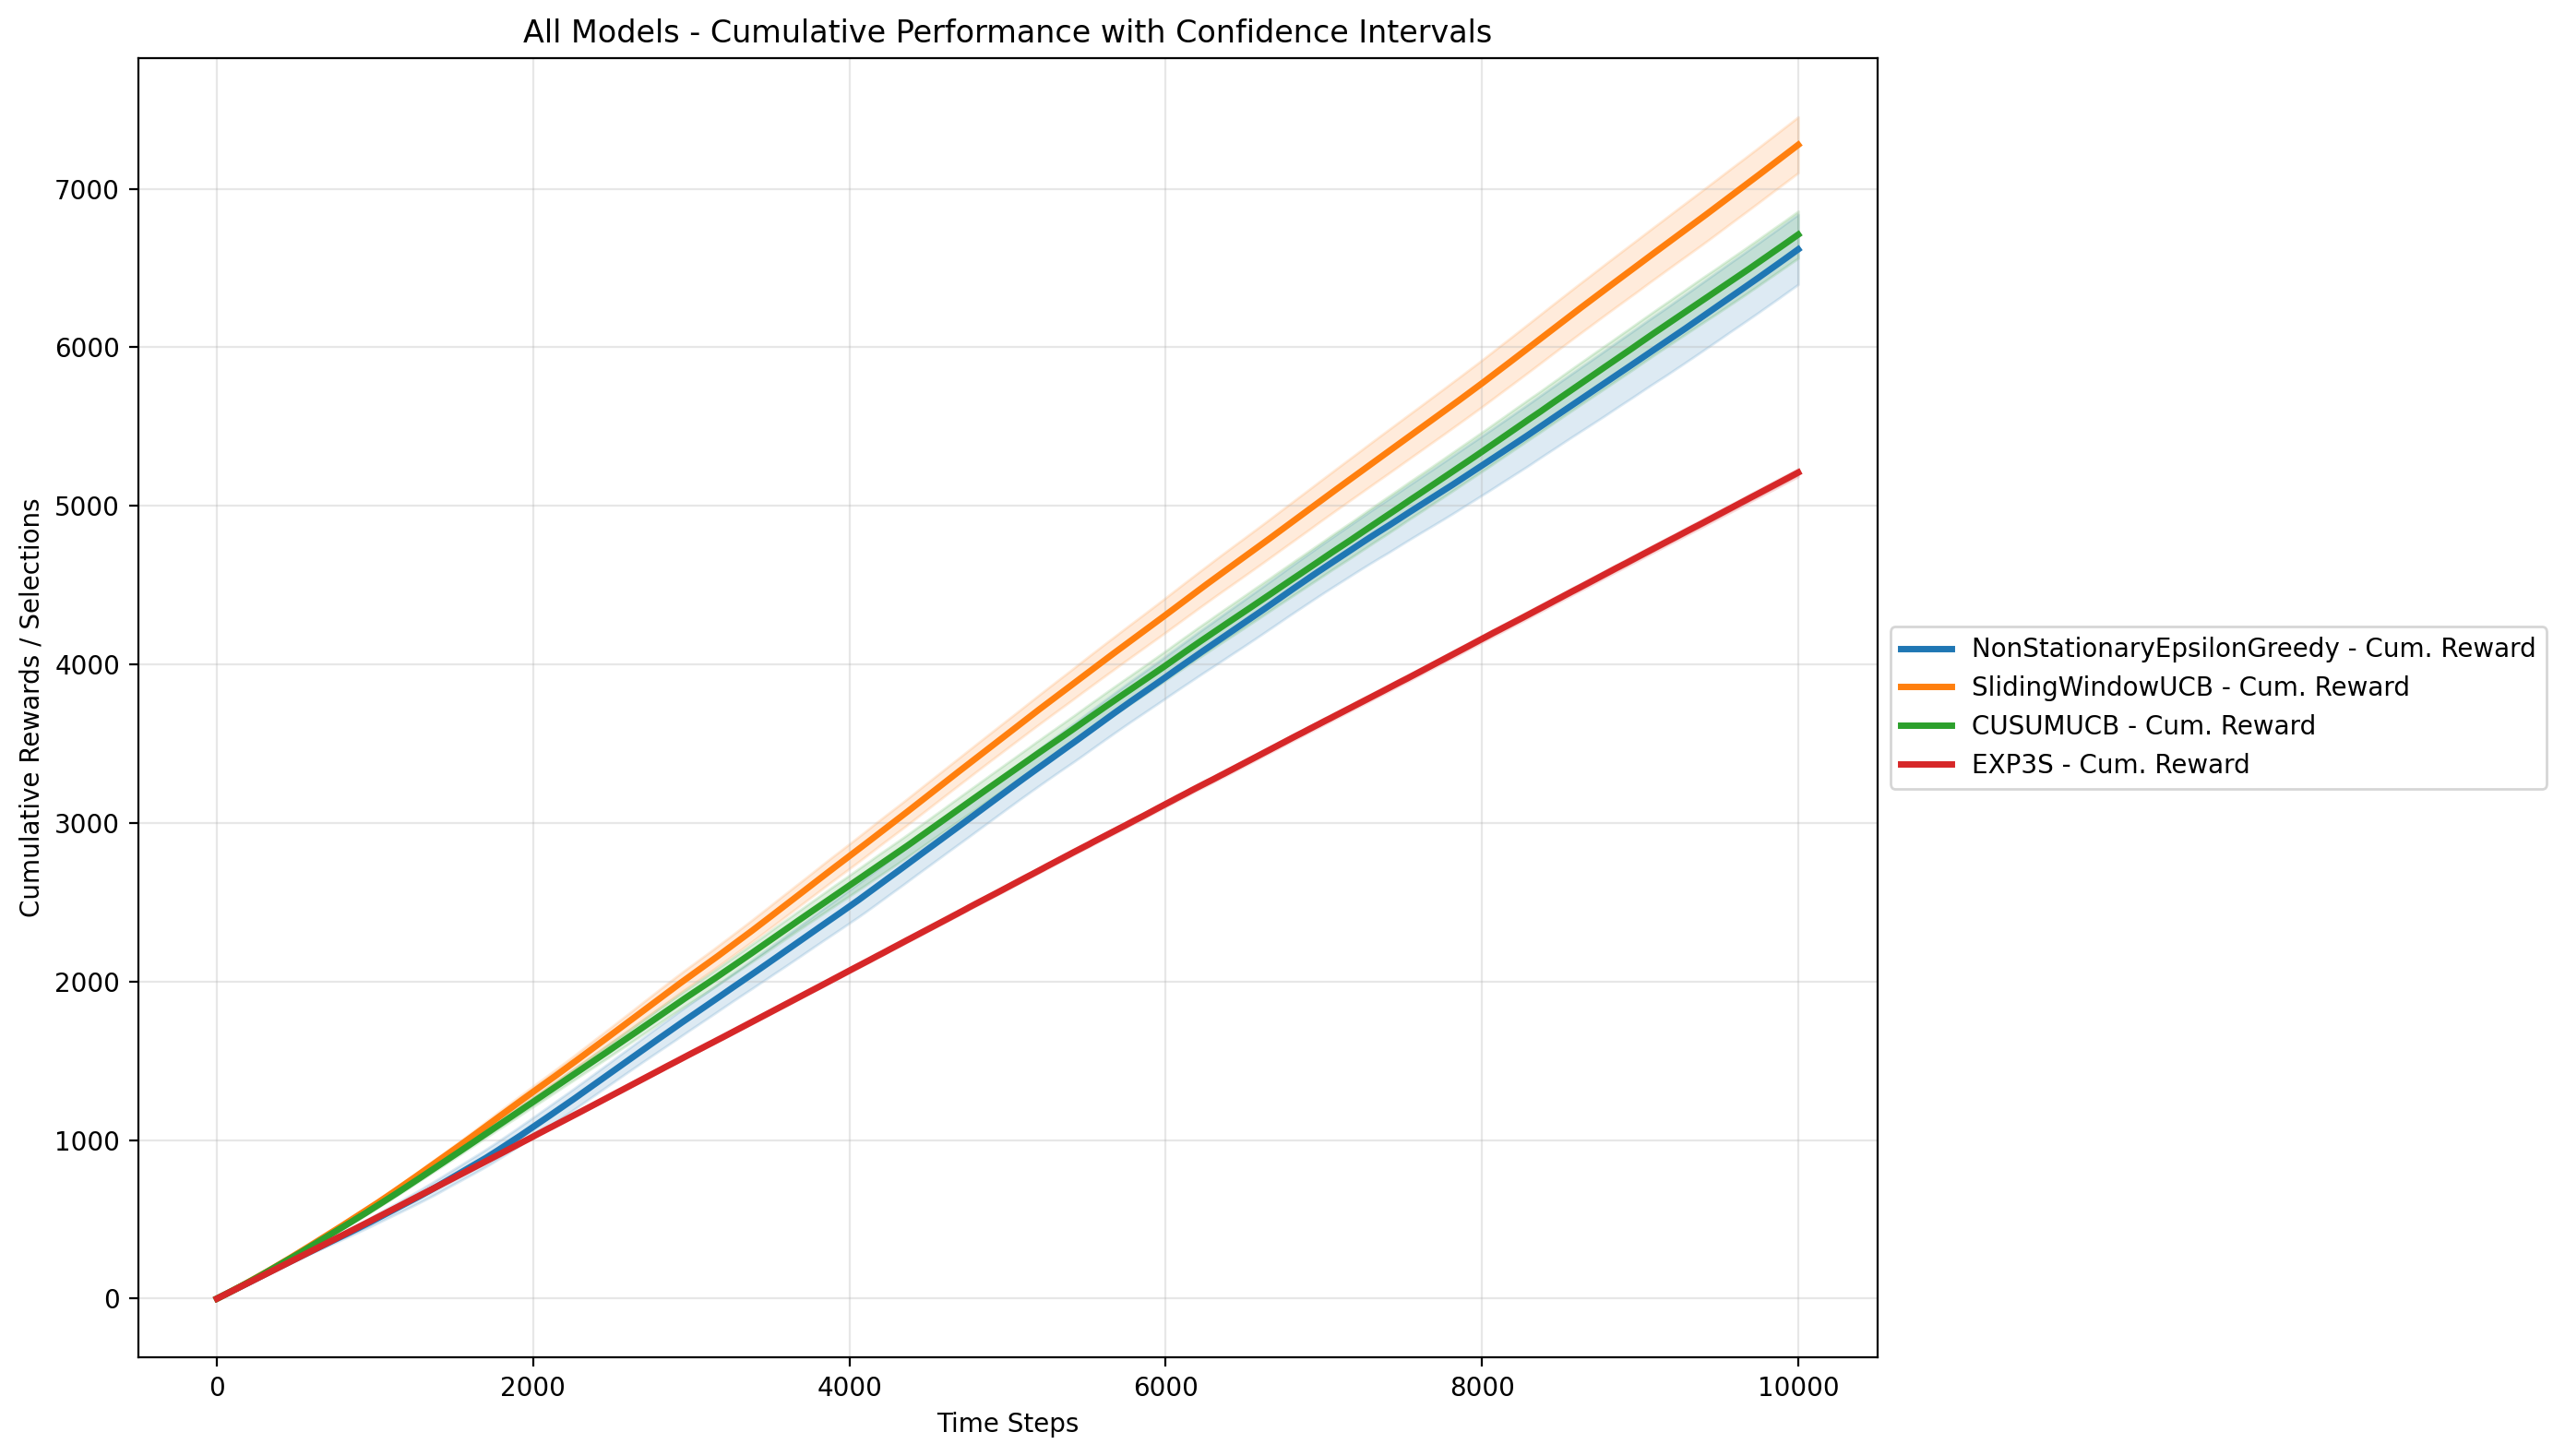
\includegraphics[width=\linewidth]{Fig/model_cumulative_all_ci.png}
        \caption{Mean cumulative reward trajectories for all four algorithms over \(T = 10{,}000\) rounds, averaged across \(50\) runs with pointwise \(95\%\) confidence intervals.}
        \label{fig:models-cum-reward}
    \end{subfigure}

    \caption{Comparison of average and cumulative rewards for the evaluated bandit algorithms in the drifting user environment.}
    \label{fig:bandit-environment}
\end{figure}




% - One singular plot with all MODELS and their corresponding rolling rewards (use the existing plot functions) -> Area plot for 50 seeds with their corresponding confidence bound

% - One singular plot with all MODELS and their corresponding CUMULATIVE rewards (use the existing plot functions) -> Area plot for 50 seeds with their corresponding confidence bound
\section{Discussion}\label{sec5}

The empirical results highlight clear differences in how the four algorithms cope
with gradual drift in user preferences. In the drifting environment, the rolling
average rewards show that SlidingWindowUCB adapts most quickly and maintains the
highest steady-state performance, which is consistent with its design choice of
discarding stale observations via a finite window. CUSUM-UCB also benefits from
its explicit change-detection mechanism, recovering rapidly after shifts but
exhibiting slightly more variability due to exploratory resets. The
Non-Stationary $\varepsilon$-Greedy baseline eventually tracks the dominant arm,
yet its constant step-size update reacts more slowly than the targeted mechanisms
in SW-UCB and CUSUM-UCB.

EXP3.S behaves differently because it is rooted in the adversarial bandit
formulation, where rewards are viewed as an arbitrary sequence rather than
independent draws from fixed probability distributions. In this paradigm the
algorithm maintains exponential weights over arms and samples actions from a
mixture of the normalized weights and a uniform exploration distribution,
similar in spirit to an entropy-regularized or softmax policy. Only the arm
played at each round receives a non-zero importance-weighted reward estimate,
so the corresponding weight is updated while the others remain unchanged. This
update structure implicitly favors previously selected actions and is well
suited to worst-case regret guarantees, but in the smoothly drifting stochastic
environment considered here it leads to conservative adaptation and lower
average reward than the stochastic baselines.

\section{Conclusion}\label{sec6}

This work introduced a reproducible simulation framework for studying user drift
through a non-stationary multi-armed bandit lens and used it to compare four
adaptive bandit algorithms. By representing users as drifting preference
vectors over content categories, the framework isolates the effect of evolving
interests while keeping the interaction model intentionally simple. Within this
environment, SlidingWindowUCB consistently achieved the highest average and
cumulative rewards, with CUSUM-UCB and Non-Stationary $\varepsilon$-Greedy
forming a competitive middle tier and EXP3.S lagging behind.

These findings indicate that lightweight stochastic methods that explicitly
discount or reset outdated information are well suited to recommendation
scenarios where preferences drift gradually over time. In contrast,
adversarially oriented algorithms such as EXP3.S may sacrifice efficiency when
the true source of non-stationarity is user behavior rather than hostile
perturbations. The proposed framework and code base can serve as a testbed for
future adaptive bandit designs and for evaluating robustness–efficiency
trade-offs under controlled forms of drift.

\subsection{Limitations}\label{sec6-1}

The experimental setup focuses on a single-user, two-arm setting with a specific
Gaussian drift process, which simplifies interpretation but does not capture the
full complexity of real recommender systems. The user’s latent preferences
evolve according to a synthetic and symmetric noise process without contextual features,
feedback loops, or heterogeneous user populations. Moreover, hyperparameters for
each algorithm were chosen using reasonable defaults rather than systematic
tuning, so the reported ranking may change under different optimization
criteria, time horizons, or drift regimes.

Another limitation is that the evaluation uses only reward-based metrics
(average and cumulative reward) and does not consider complementary notions such
as dynamic regret with respect to a time-varying oracle, fairness across arms,
or robustness to model misspecification. The conclusions are therefore
conditional on the specific reward structure and drift dynamics encoded in the
simulator, and care must be taken when extrapolating to production systems with
richer feedback and business constraints.

\subsection{Future Scope}\label{sec6-2}

Several directions can extend this work. First, the drifting environment can be
generalized to multi-user and multi-category settings with contextual
information, enabling the study of contextual and linear bandit algorithms under
user drift. Second, future experiments could incorporate abrupt regime changes,
seasonality, or mixed stochastic–adversarial reward sequences to test whether
the relative advantages of SW-UCB, CUSUM-UCB, and EXP3.S persist under more
challenging dynamics. Third, a systematic hyperparameter search and sensitivity
analysis would clarify how robust the observed performance ordering is to design
choices such as window length, CUSUM thresholds, and exploration rates.

Beyond simulation, the framework could be adapted for offline evaluation using
historical interaction logs, for example via inverse propensity scoring or
counterfactual estimators, to bridge the gap between synthetic and real-world
data. Integrating additional objectives—such as diversity, fairness, or risk
control—would also allow the comparison of adaptive bandit algorithms along
multiple axes that matter in deployed recommender systems.
%%===========================================================================================%%
%% If you are submitting to one of the Nature Portfolio journals, using the eJP submission   %%
%% system, please include the references within the manuscript file itself. You may do this  %%
%% by copying the reference list from your .bbl file, paste it into the main manuscript .tex %%
%% file, and delete the associated \verb+\bibliography+ commands.                            %%
%%===========================================================================================%%

\bibliography{sn-bibliography}% common bib file
%% if required, the content of .bbl file can be included here once bbl is generated
%%\input sn-article.bbl

\end{document}
